\documentclass[10pt, aspectratio = 169, handout]{beamer} % handout

\usepackage{amsmath}
\usepackage{fontawesome} 
\usepackage{ragged2e}
\usepackage{color}
\usepackage{tikz}
\usepackage{soul}
\usepackage{xcolor}
\usepackage{import}
\usepackage{xifthen}
\usepackage{pdfpages}
\usepackage{transparent}
\usepackage{soul}
\usepackage[mathscr]{euscript}

\usetikzlibrary{shapes, backgrounds, plotmarks}

% Curly D [euscript]
\DeclareSymbolFont{rsfs}{U}{rsfs}{m}{n}
\DeclareSymbolFontAlphabet{\mathscrsfs}{rsfs}

\usetheme[]{metropolis}
\usecolortheme[]{wolverine}

\usefonttheme{serif}
\setbeamercovered{transparent = 0.5}

\setbeamertemplate{theorems}[numbered]

\definecolor{title-bg}{RGB}{240, 240, 240}
\definecolor{title-fg}{RGB}{128, 113, 93}
\definecolor{my-red}{RGB}{254, 132, 135}
\definecolor{my-blue}{RGB}{59, 180, 252}
\definecolor{my-green}{RGB}{125, 221, 149}
\definecolor{titles}{RGB}{0, 0, 122}
\setbeamercolor{block title}{fg = title-fg, bg = title-bg}
\setbeamercolor{header-color}{fg = title-fg, bg = title-bg}
\setbeamercolor{background canvas}{bg = white}

\let\oldtextbf\textbf
\renewcommand\textbf[1]{\textcolor{titles}{\oldtextbf{#1}}}

\setbeamertemplate{footline}{%
	\leavevmode%
	\hbox{%
		\begin{beamercolorbox}[wd = 0.800\textwidth, ht = 4ex, dp = 2ex, left]{}%
			\hspace{4pt} \texttt{Model-based Geostatistics under Spatially Varying Preferential Sampling}
		\end{beamercolorbox}%
		\begin{beamercolorbox}[wd = 0.120\textwidth, ht = 4ex, dp = 2ex, center]{}%
			\raisebox{-1pt}{\insertslidenavigationsymbol~\insertsectionnavigationsymbol}
		\end{beamercolorbox}%
		\begin{beamercolorbox}[wd = 0.080\textwidth, ht = 4ex, dp = 2ex, center]{}%
			\texttt{\insertframenumber~/~\inserttotalframenumber}
		\end{beamercolorbox}%
	}%
}%



\author{André Victor Ribeiro Amaral}

\begin{document}
	\AtBeginSection{}
	\metroset{block = fill}
	{
		\usebackgroundtemplate{
    		\hspace{6pt}
    		
\includegraphics[width=0.35\textwidth]{Images/KAUST_logo.png}
    		\hspace{212pt}
    		\raisebox{-6pt}{
\includegraphics[width=0.225\textwidth]{Images/JSM_logo.png}}
		}

        \begin{frame}[t]
            
            \centering
            \vspace{65pt}
            \textbf{{\large \usebeamercolor[fg]{frametitle}Model-based Geostatistics under Spatially Varying Preferential Sampling}} \\
            \vspace{15pt}
            {\normalsize André V.\hspace{1pt} Ribeiro Amaral${}^{\hspace{-1pt}~\dagger}$}\\
            {\scriptsize\texttt{\href{mailto:andre.ribeiroamaral@kaust.edu.sa}{andre.ribeiroamaral@kaust.edu.sa}}} \\
            \vspace{15pt}
            {\small King Abdullah University of Science and Technology}\\
            {\small Geospatial Statistics and Health Surveillance Research Group} \\ \vspace{15pt}

            \begin{flushleft} 
            {\small ${}^{\dagger\hspace{1pt}}$Joint work with Elias T. Krainski, Ruiman Zhong, and Paula Moraga.}
            \end{flushleft}
        \end{frame}
  	}

	\begin{frame}[t]
		\frametitle{Introduction}
		\justifying

        In this work, we propose a \textbf{new model} for \textbf{geostatistical data} that accounts for \textbf{preferential sampling} by including a \textbf{spatially varying coefficient} that describes the dependence strength between the process that models the sampling locations and the latent field. \vspace{12pt}

        \pause

        Here, \textbf{geostatistics} will refer to the analysis of data sampled from a process $\zeta(x)$ in a spatially continuous domain, say $\mathscrsfs{D}$, at a discrete set of locations $x = (x_1, \cdots, x_n)^{\top}$, such that $x_i \in \mathscrsfs{D}$, $\forall i$. \vspace{12pt}

        \pause

        Let $\xi$ be the point process that models the locations where the process $\zeta$ is observed, then if
        \begin{align*}
            \pi(\zeta, \xi) \neq \pi(\zeta) \cdot \pi(\xi),
        \end{align*}
        where $\pi(x)$ means ``distribution of $x$,'' we say that we are under a \textbf{``preferential sampling''} setting. Otherwise, we are are under a ``non-preferential sampling'' setting.
	\end{frame}

	
	  \begin{frame}[t]
		\frametitle{Preferential Sampling Model (Diggle et al., 2010)}
		\justifying

       Suppose that $y_i$ denotes the observed value of a noisy version of the spatial process $\zeta(x_i)$ at a given location $x_i$, for any $i$. Then, the following approach is a common choice
        \begin{align*} 
        	y_i = \mu + \zeta(x_i) + \epsilon_i, \text{ s.t. } \epsilon_i \overset{\text{i.i.d.}}{\sim} \text{Normal}(0, \sigma^2_{\epsilon}) 
        \end{align*}
        Here, we can assume that $\zeta(x_i)$ has mean zero. In that case, $\mathbb{E}(y_i) = \mu$, $\forall i \in \{1, \cdots, n\}$. \vspace{12pt}

        \pause

        Aiming to allow for the stochastic dependence between $\xi$ and $\zeta$, we will assume the following \vspace{-12pt}
        \begin{enumerate} \justifying
        	\item $\zeta$ is a stationary and isotropic Gaussian random process with mean zero, variance $\sigma^2_{\zeta}$, and covariance function $r_{\zeta}(h; \theta)$, where $h = ||x_1 - x_2||$ is the Euclidean distance between $x_1$ and $x_2$. \pause
        	\item $\xi|\zeta(x)$ is a PP with intensity $\lambda(x) = \exp\{\alpha + \gamma \cdot \zeta(x)\}$, such that $x \in \mathscrsfs{D}$, and $\alpha, \gamma \in \mathbb{R}$. \pause
        	\item Conditional on $x$ and $\zeta(x)$, $y = (y_1, \cdots, y_n)^{\top}$ is an i.i.d$.$ vector, such that $y_i \sim \text{Normal}(\mu + \zeta(x_i), \sigma^2_{\epsilon})$, $\forall i$.
        \end{enumerate}
	\end{frame}

	  \begin{frame}[t]
		\frametitle{\textcolor{red}{Extended} Preferential Sampling Model}
		\justifying

        To allow for a \textbf{spatially varying degree of preferentiality,} instead of assumption ``2.'' as before, we will say that $\xi|\zeta(x)$ is a PP with intensity 
        \begin{align} \label{eq:lambda-assumption}
            \lambda(x) = \exp\{\alpha + \gamma(x) \cdot \zeta(x)\},
        \end{align}
        where $x \in \mathscrsfs{D}$, and $\alpha, \gamma(x) \in \mathbb{R}$. Here, \ul{$\gamma(x)$ is a process defined on $\mathscrsfs{D}$ that dictates how the degree of preferentiality must vary over the spatial domain}. For now, we will not impose any constraints over $\gamma(x)$.  \vspace{12pt}

        \pause

        However, from Equation \eqref{eq:lambda-assumption}, notice that the multiplicative structure for the preferentiality and latent fields may yield identifiability issues. \textbf{\textcolor{red}{This might be a problem!}}
	\end{frame}

	  \begin{frame}[t]
		\frametitle{\textcolor{red}{Extended} Preferential Sampling Model}
		\justifying

        To alleviate this issue, we will specify $\gamma(x)$ using a (typically small)  set of basis functions in the following way
        \begin{align*}
            \hat{\gamma}(x) = \sum_{k = 1}^{K}\beta_k \phi_k(x),
        \end{align*}
        where $\beta_k \in \mathbb{R}$, for all $k \in \{1, \cdots, K\}$, are uncorrelated Gaussian distributed coefficients, and $\{\phi_k(x)\}_{k = 1}^K$ is a set of basis function (examples come next) defined over the same domain\hspace{-1pt} $\mathscrsfs{D}$. 
        
	\end{frame}

	  \begin{frame}[t]
		\frametitle{\textcolor{red}{Extended} Preferential Sampling Model}
		\justifying

        Thus, the complete model is specified as follows
        \begin{align} \label{eq:full-model}
        	y_i &= \mu + \zeta(x_i) + \epsilon_i, \text{ s.t. } \epsilon_i \overset{\text{i.i.d.}}{\sim} \text{Normal}(0, \sigma^2_{\epsilon}),~\forall i \\ 
            \zeta(x) &\sim \text{Gaussian Process}(0, r_\zeta(h; \theta)) \nonumber \\ 
            \xi|\zeta(x) &\sim \text{Poisson Point Process}(\lambda(x)) \nonumber \\ 
            \lambda(x) &= \exp\{\alpha + \gamma(x) \cdot \zeta(x)\} \nonumber \\ 
            \gamma(x) &= \sum_{k = 1}^{K}\beta_k \phi_k(x), \text{ s.t. } \beta_k \overset{\text{i.i.d.}}{\sim} \text{Normal}(0, \sigma^2_{\beta}),~\forall k, \nonumber
        \end{align}
        where the covariance function $r_\zeta(h; \theta)$ will be defined based on the Matérn model.
	\end{frame}

 	  \begin{frame}[t]
		\frametitle{Basis Functions}
		\justifying

        One might consider different types of \textbf{basis functions}---e.g., \ul{constant}, \ul{piecewise constant}, (horizontal or vertical) \ul{unidirectional triangular}, or \ul{radial basis} (built using a compactly supported Wendland function defined in two dimensions).

        \begin{figure}[!ht]
        	\centering
        	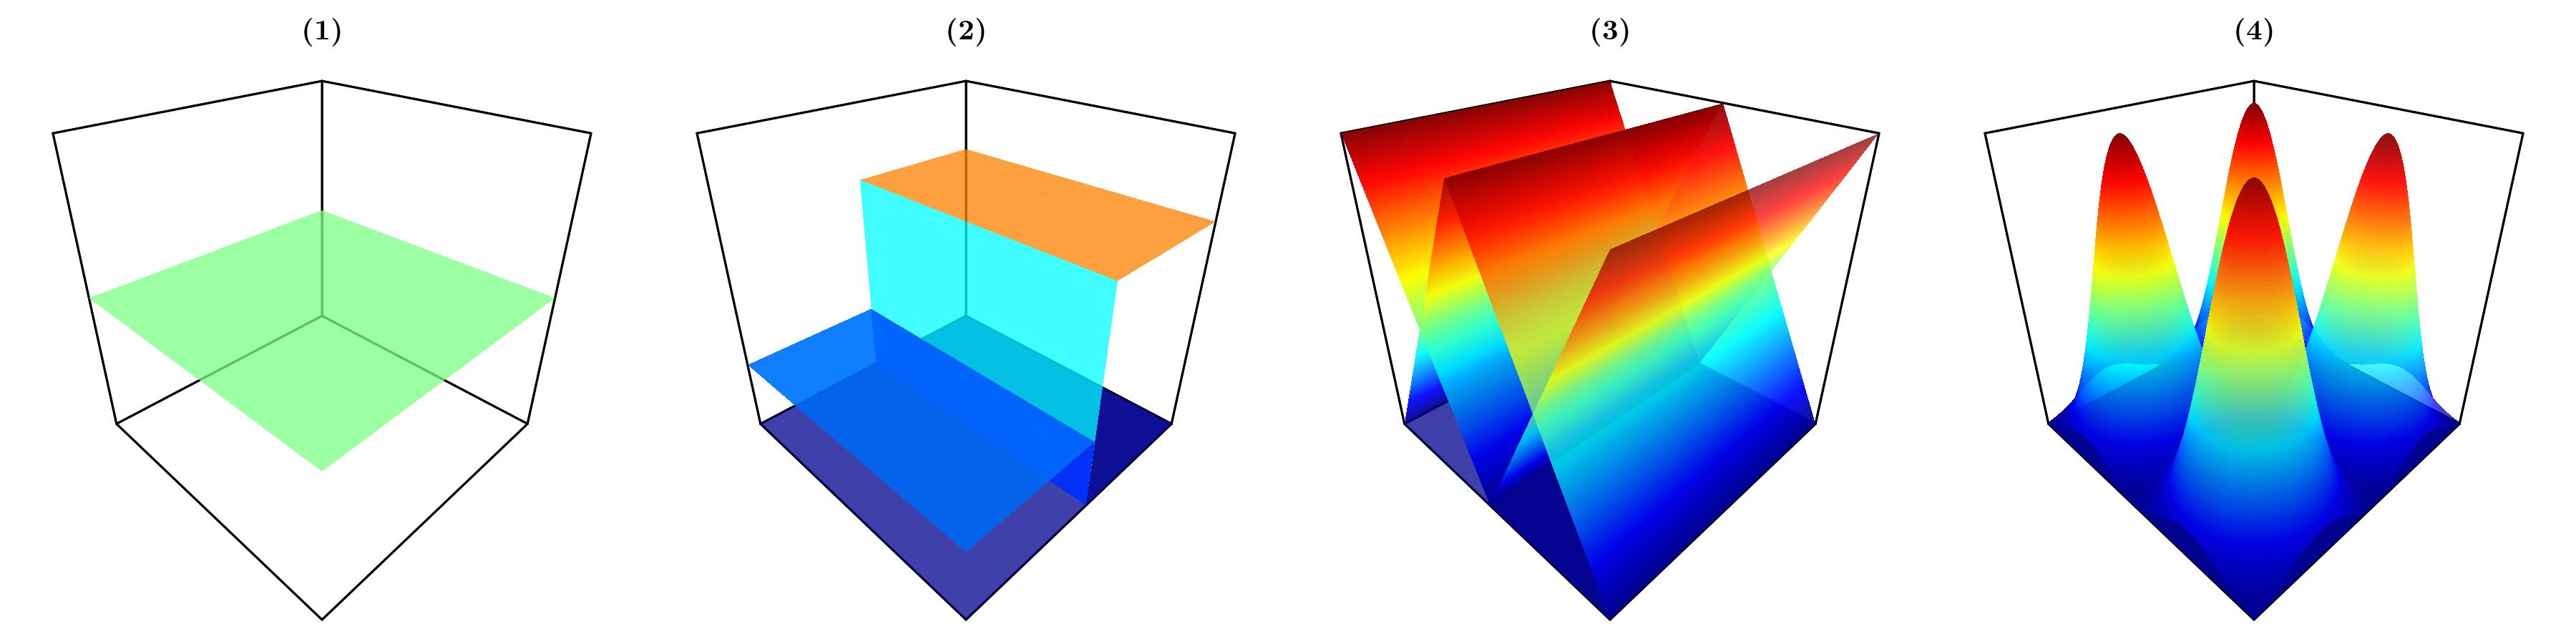
\includegraphics[width = 1\textwidth]{Images/basis-functions.jpeg}
            \caption{\justifying The basis functions were set to (1) \ul{constant}, (2) \ul{piecewise constant}, (3) horizontal \ul{unidirectional triangular}, and (4) \ul{radial basis} (Wendland).}
        	\label{fig:basis-functions}
        \end{figure}
	\end{frame}

     \begin{frame}[t]
		\frametitle{Example}
		\justifying

        \begin{figure}[!ht]
        	\centering
        	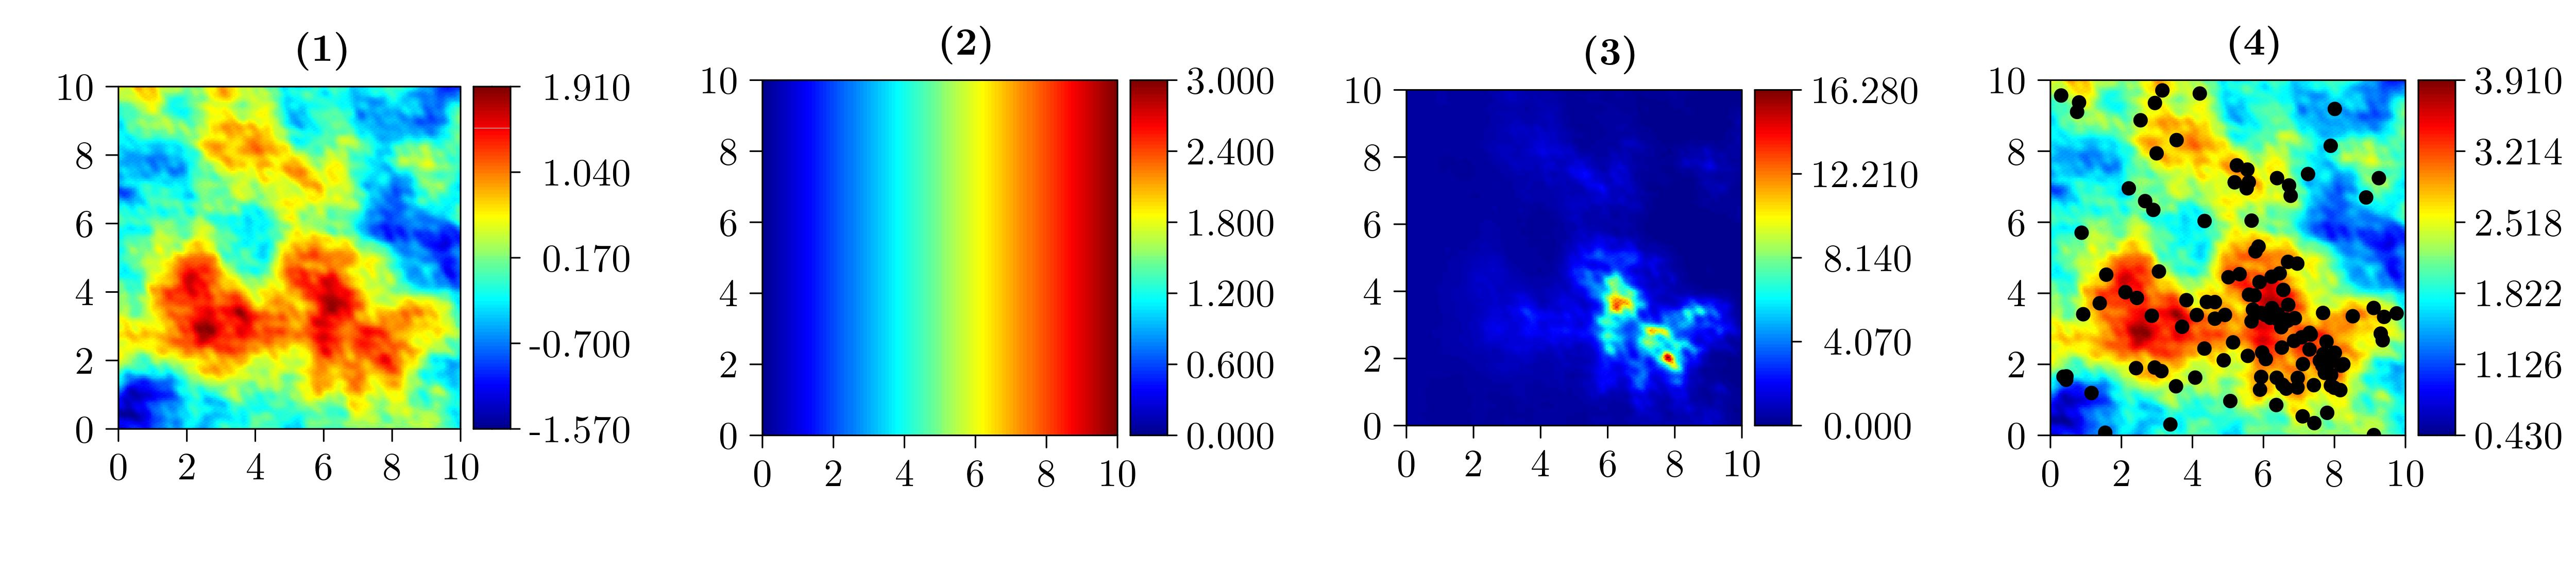
\includegraphics[width = 1\textwidth]{Images/simulated-example.jpeg}
            \caption{\justifying Simulated data in $\mathscrsfs{D} = [0, 10] \times [0,10]$ for Scenario 04 and $\mathbb{E}(N(\mathscrsfs{D})) = 100$. (1) is a realization of the latent field $\zeta(x)$, (2) is the preferentiality surface $\gamma(x)$ with scale parameter $s = 3$, (3) is the intensity process $\lambda(x)$, and (4) is $\mu + \zeta(x)$ with the observations plotted as points.}
        	\label{fig:simulated-example}
        \end{figure}
	\end{frame}

\begin{frame}[t]
        \frametitle{Application}
		\justifying

        We will model air pollution based on the $\text{PM}_{2.5}$ levels. In particular, the $\text{\textbf{PM}}_{\textbf{2.5}}$ \textbf{levels} were collected in the \textbf{USA} in 2022 and averaged across the year. In total, we have \textbf{942 stations}.

        \vspace{-6pt}

        \begin{figure}[!ht]
        	\centering
        	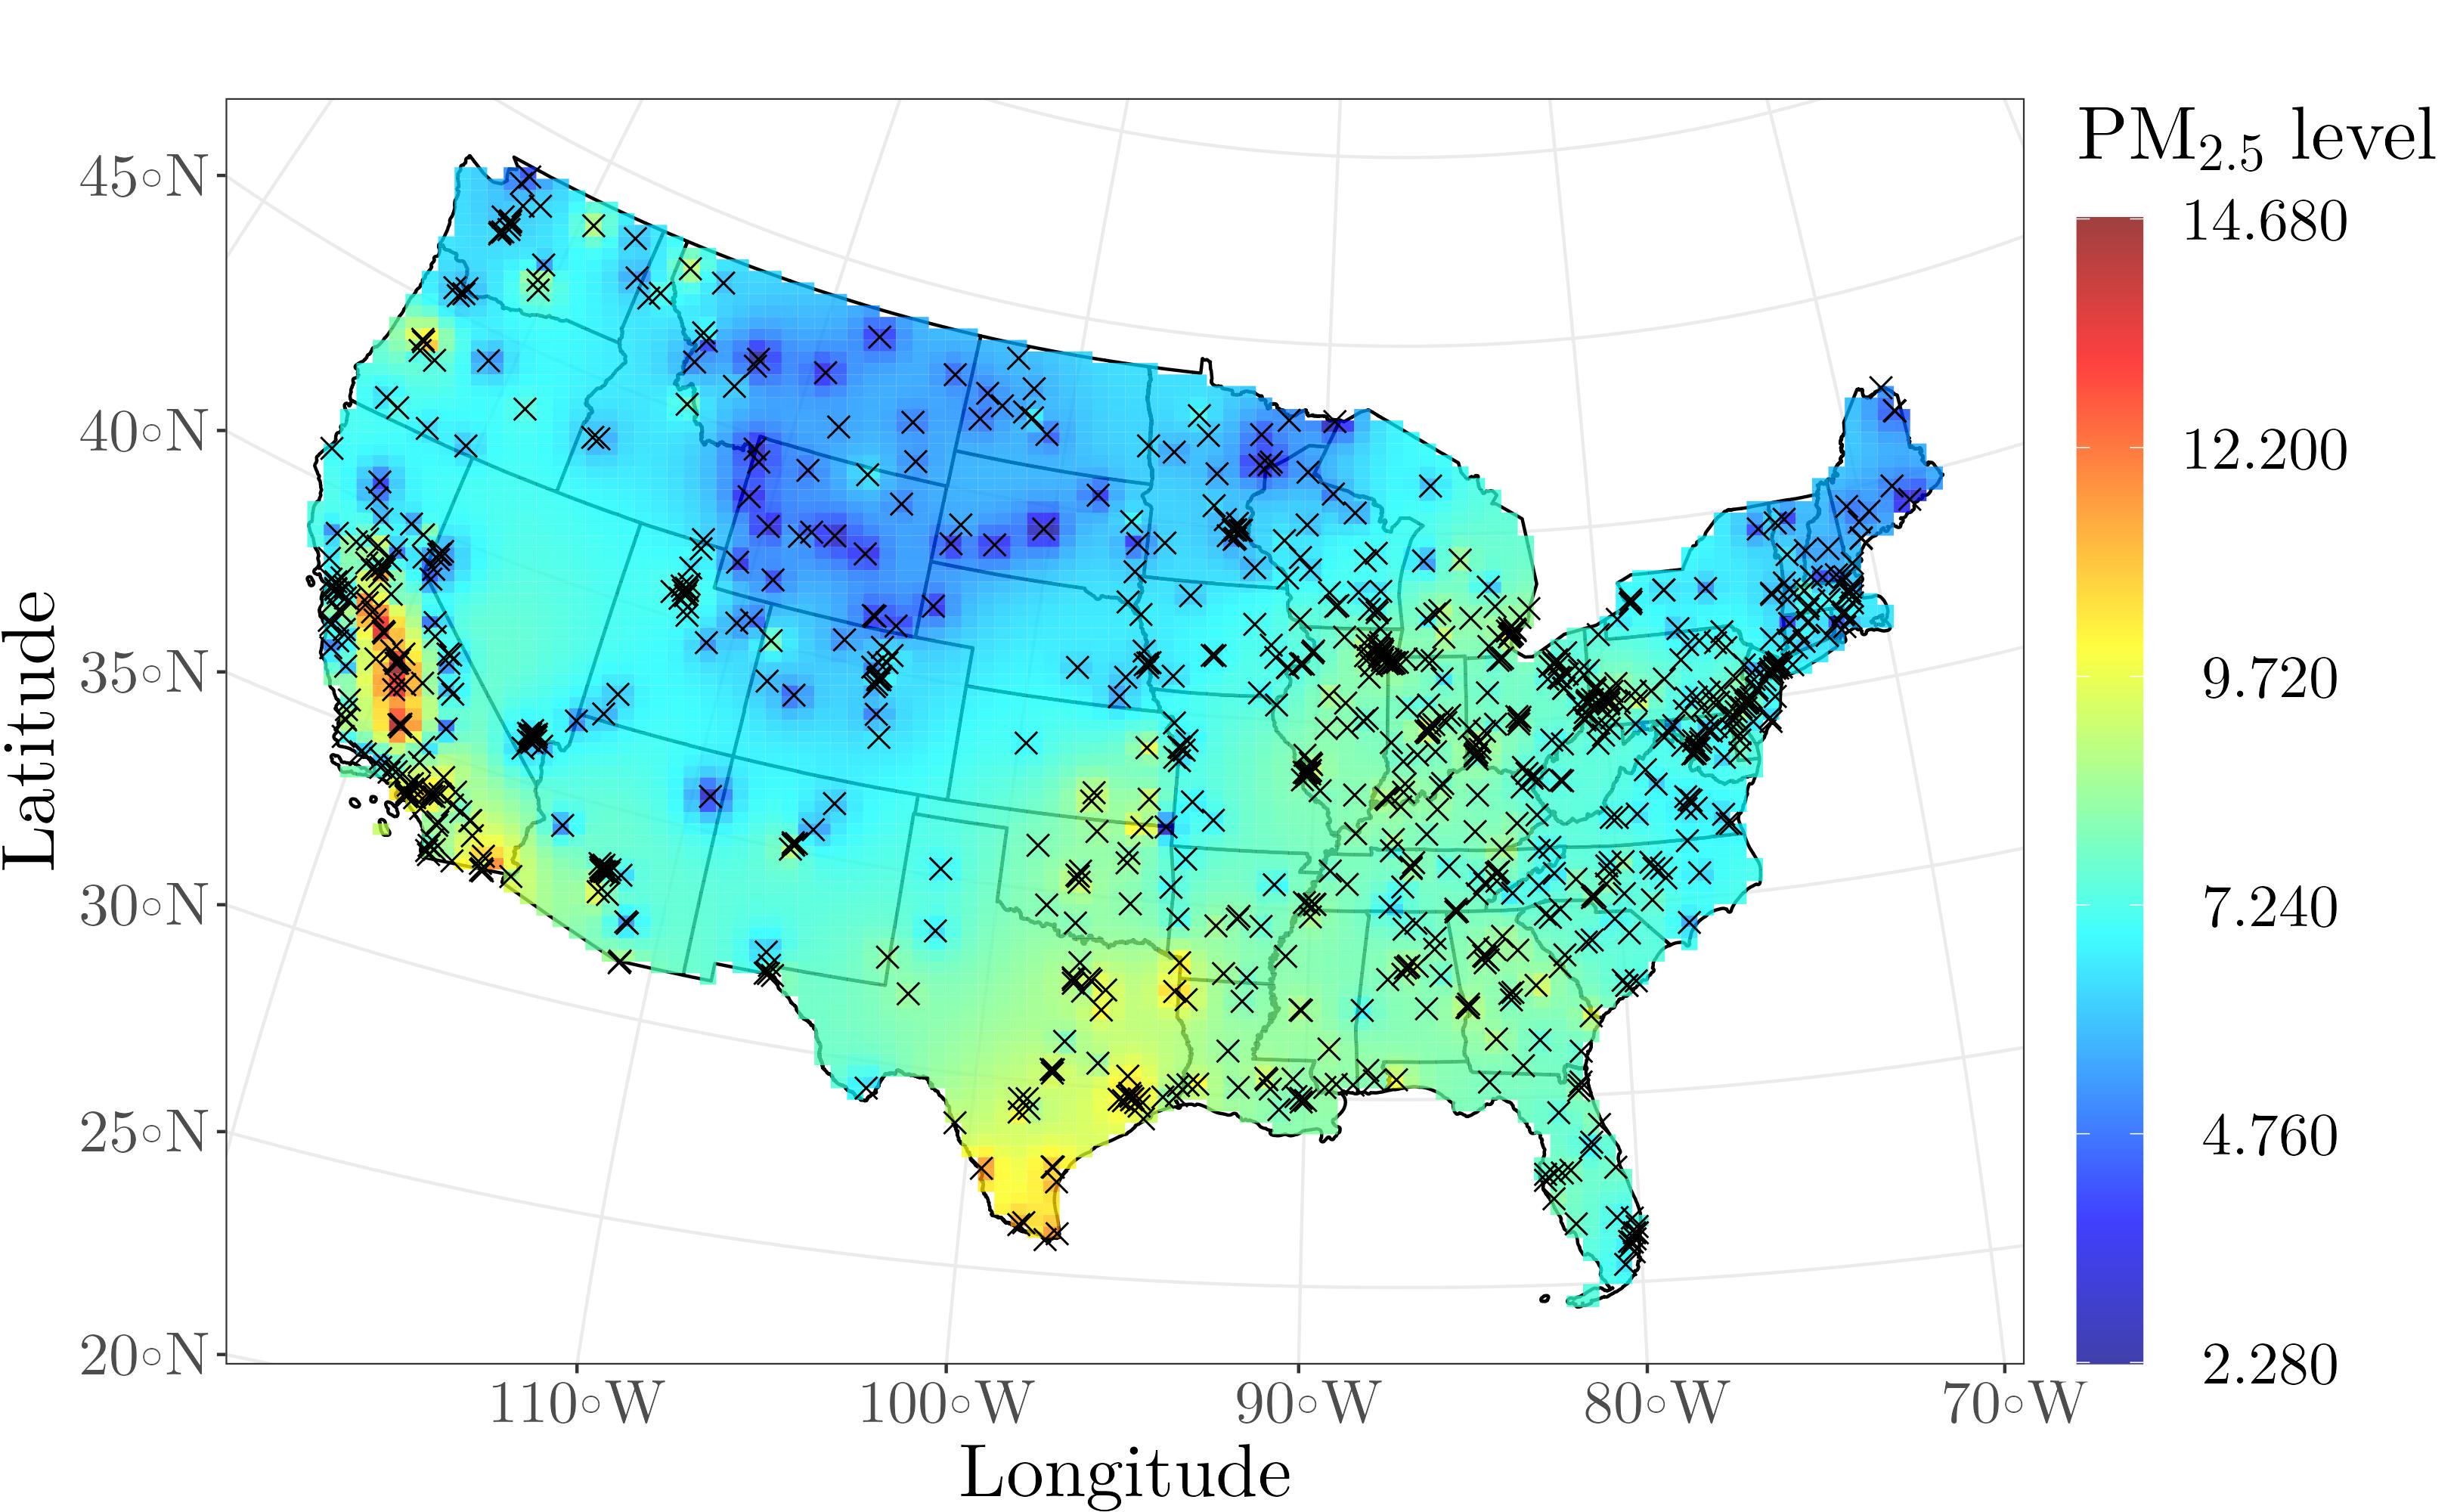
\includegraphics[width = 0.625\textwidth]{Images/free_assumptions.jpeg} \vspace{-6pt}
            \caption{\justifying Sampling locations (942 stations) and interpolated values (via IDW) for the \hspace{-1pt}$\text{PM}_{2.5}$ levels.}
        	\label{fig:usa_pm25_obs}
        \end{figure}
        
	\end{frame}

     \begin{frame}[t]
        \frametitle{Application}
		\justifying

        We will fit the ``radial basis (Wendland)''-based model, such that $K = 15$. The following map show the estimated $\textbf{PM}_{\textbf{2.5}}$ \textbf{levels} (based on the posterior mean).

        \vspace{-6pt}

        \begin{figure}[!ht]
        	\centering
        	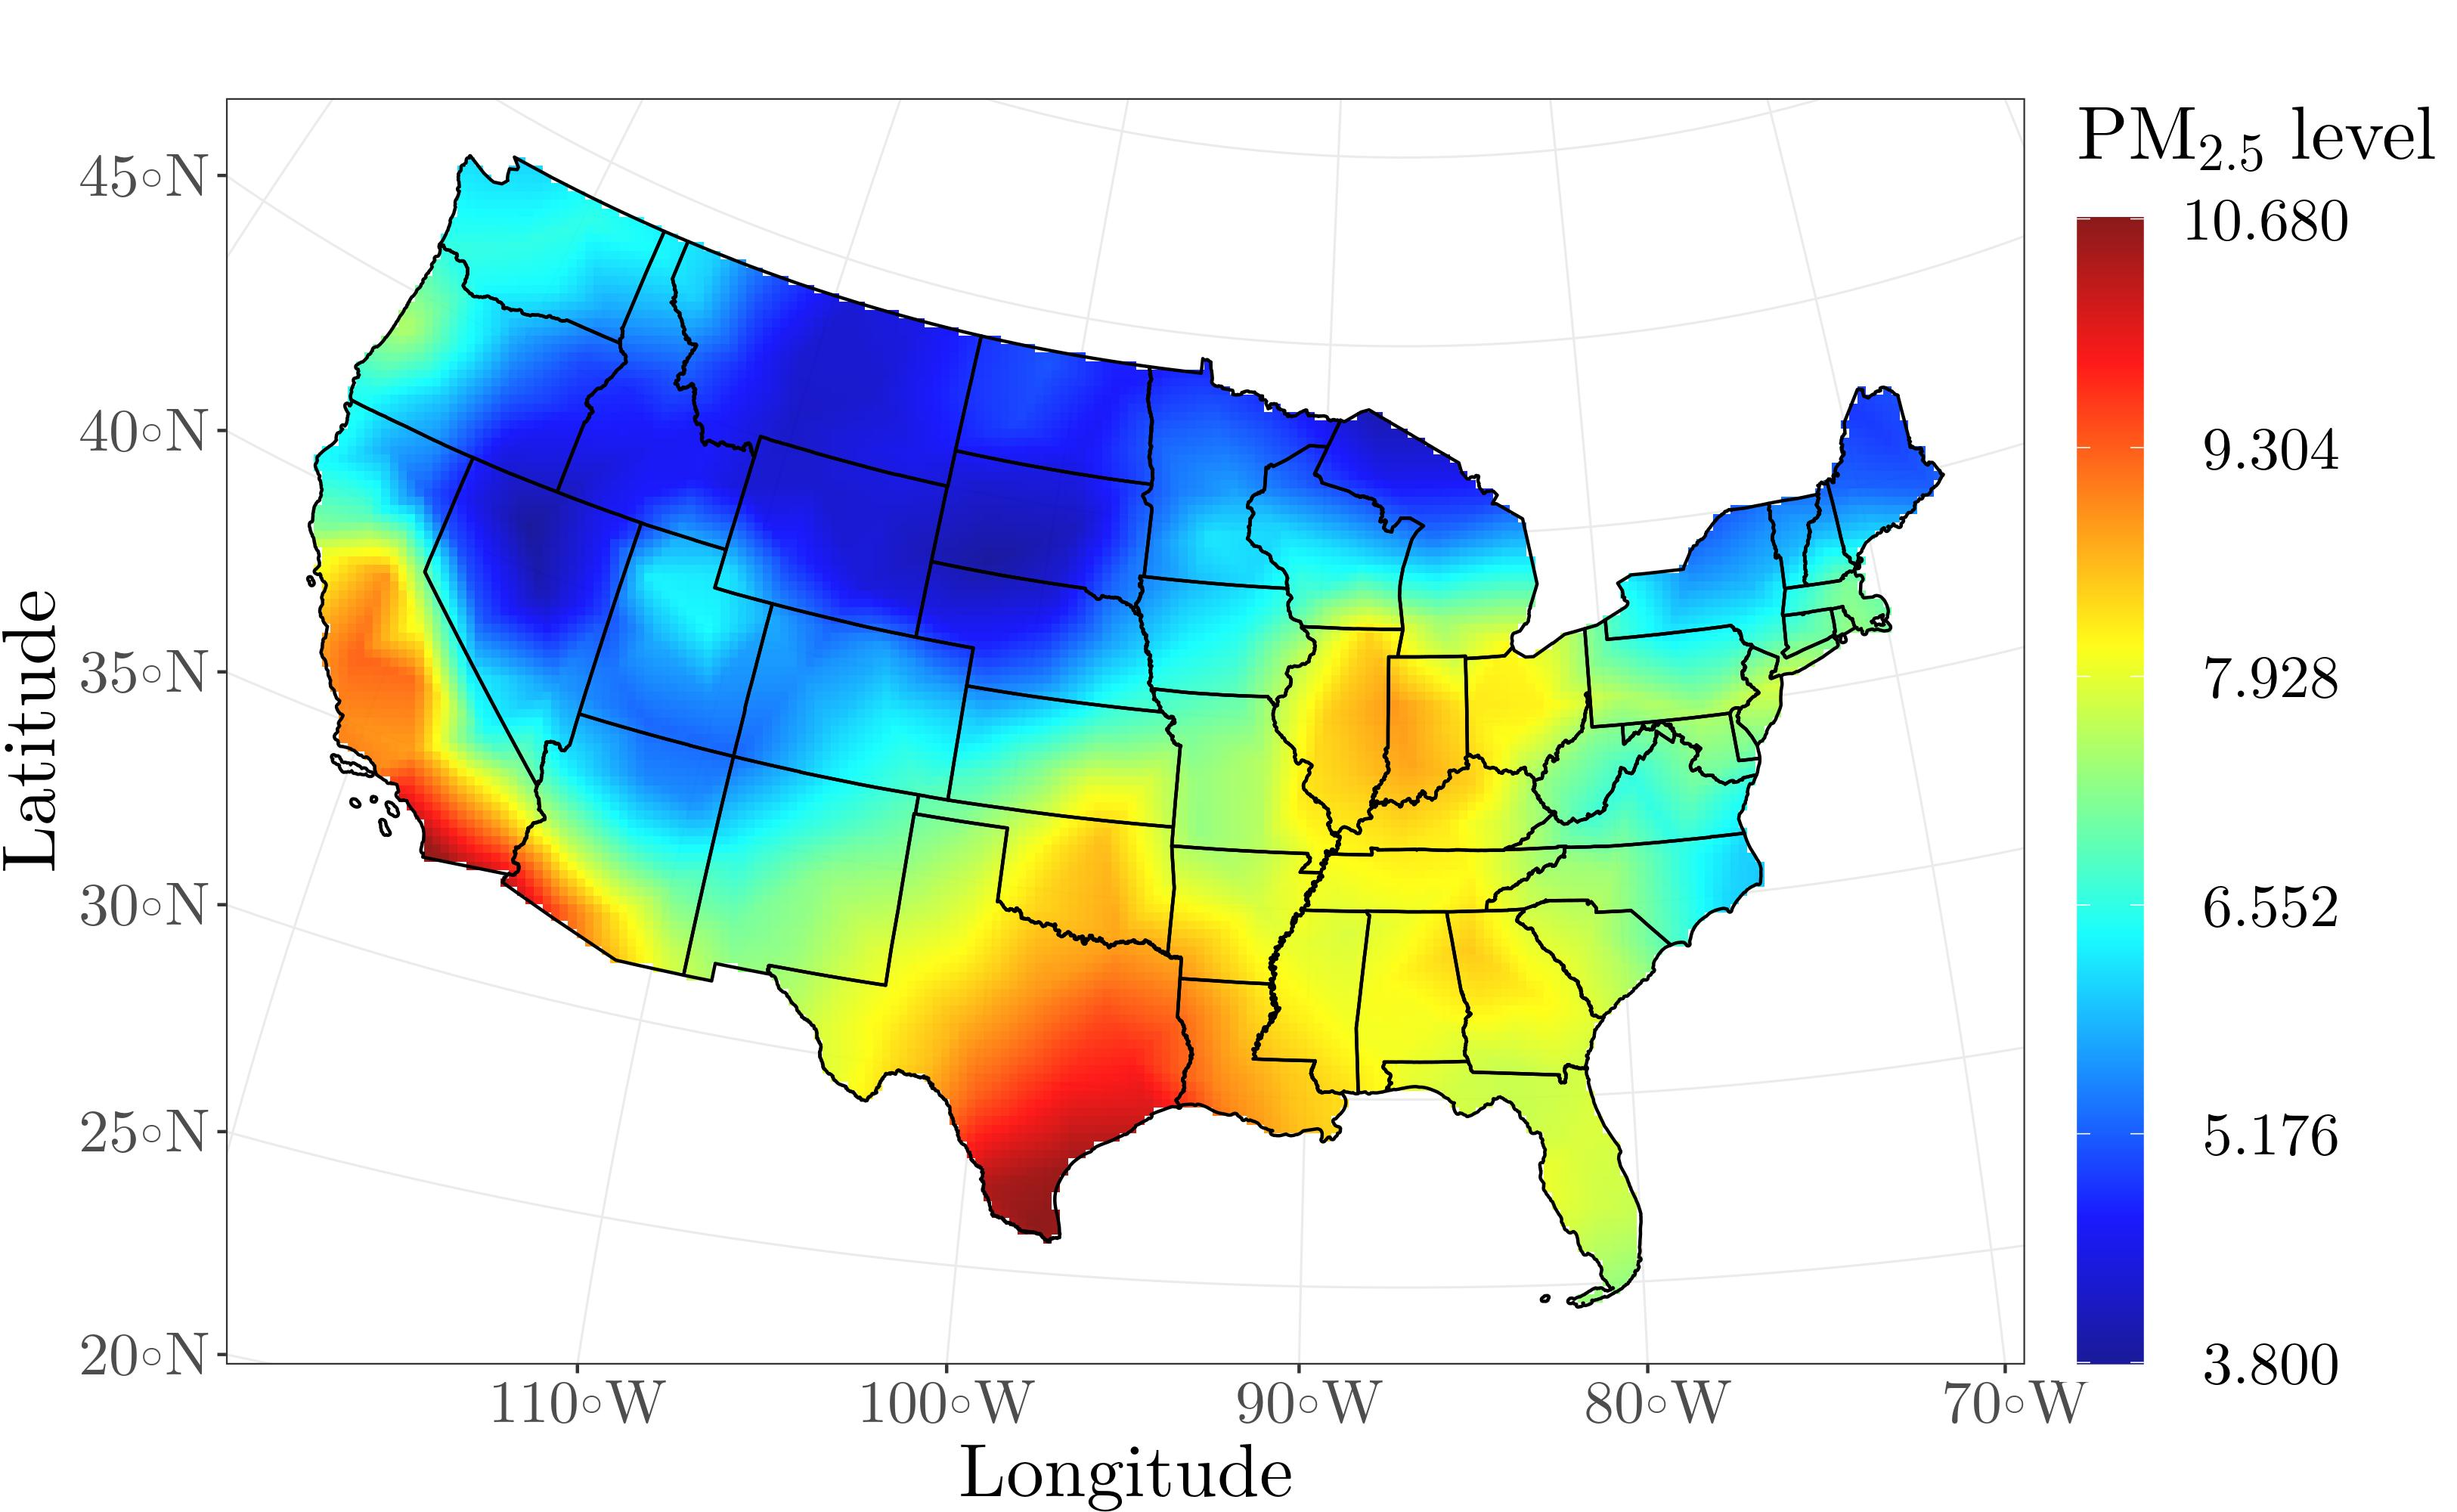
\includegraphics[width = 0.625\textwidth]{Images/usa_pm25.jpeg} \vspace{-6pt}
            \caption{\justifying Estimated $\text{PM}_{2.5}$ levels (in $\mu$g/m${}^3$) in 2022 in the $\text{USA}$ territory (excluding ``Alaska'').}
        	\label{fig:usa_pm25}
        \end{figure}

	\end{frame}

    \begin{frame}[t]
        \frametitle{Application}
		\justifying

        Under the same settings for the fitted model, we can investigate the estimated (based on the posterior mean) \textbf{preferentiality surface} $\gamma(x)$.

        \vspace{-6pt}

        \begin{figure}[!ht]
        	\centering
        	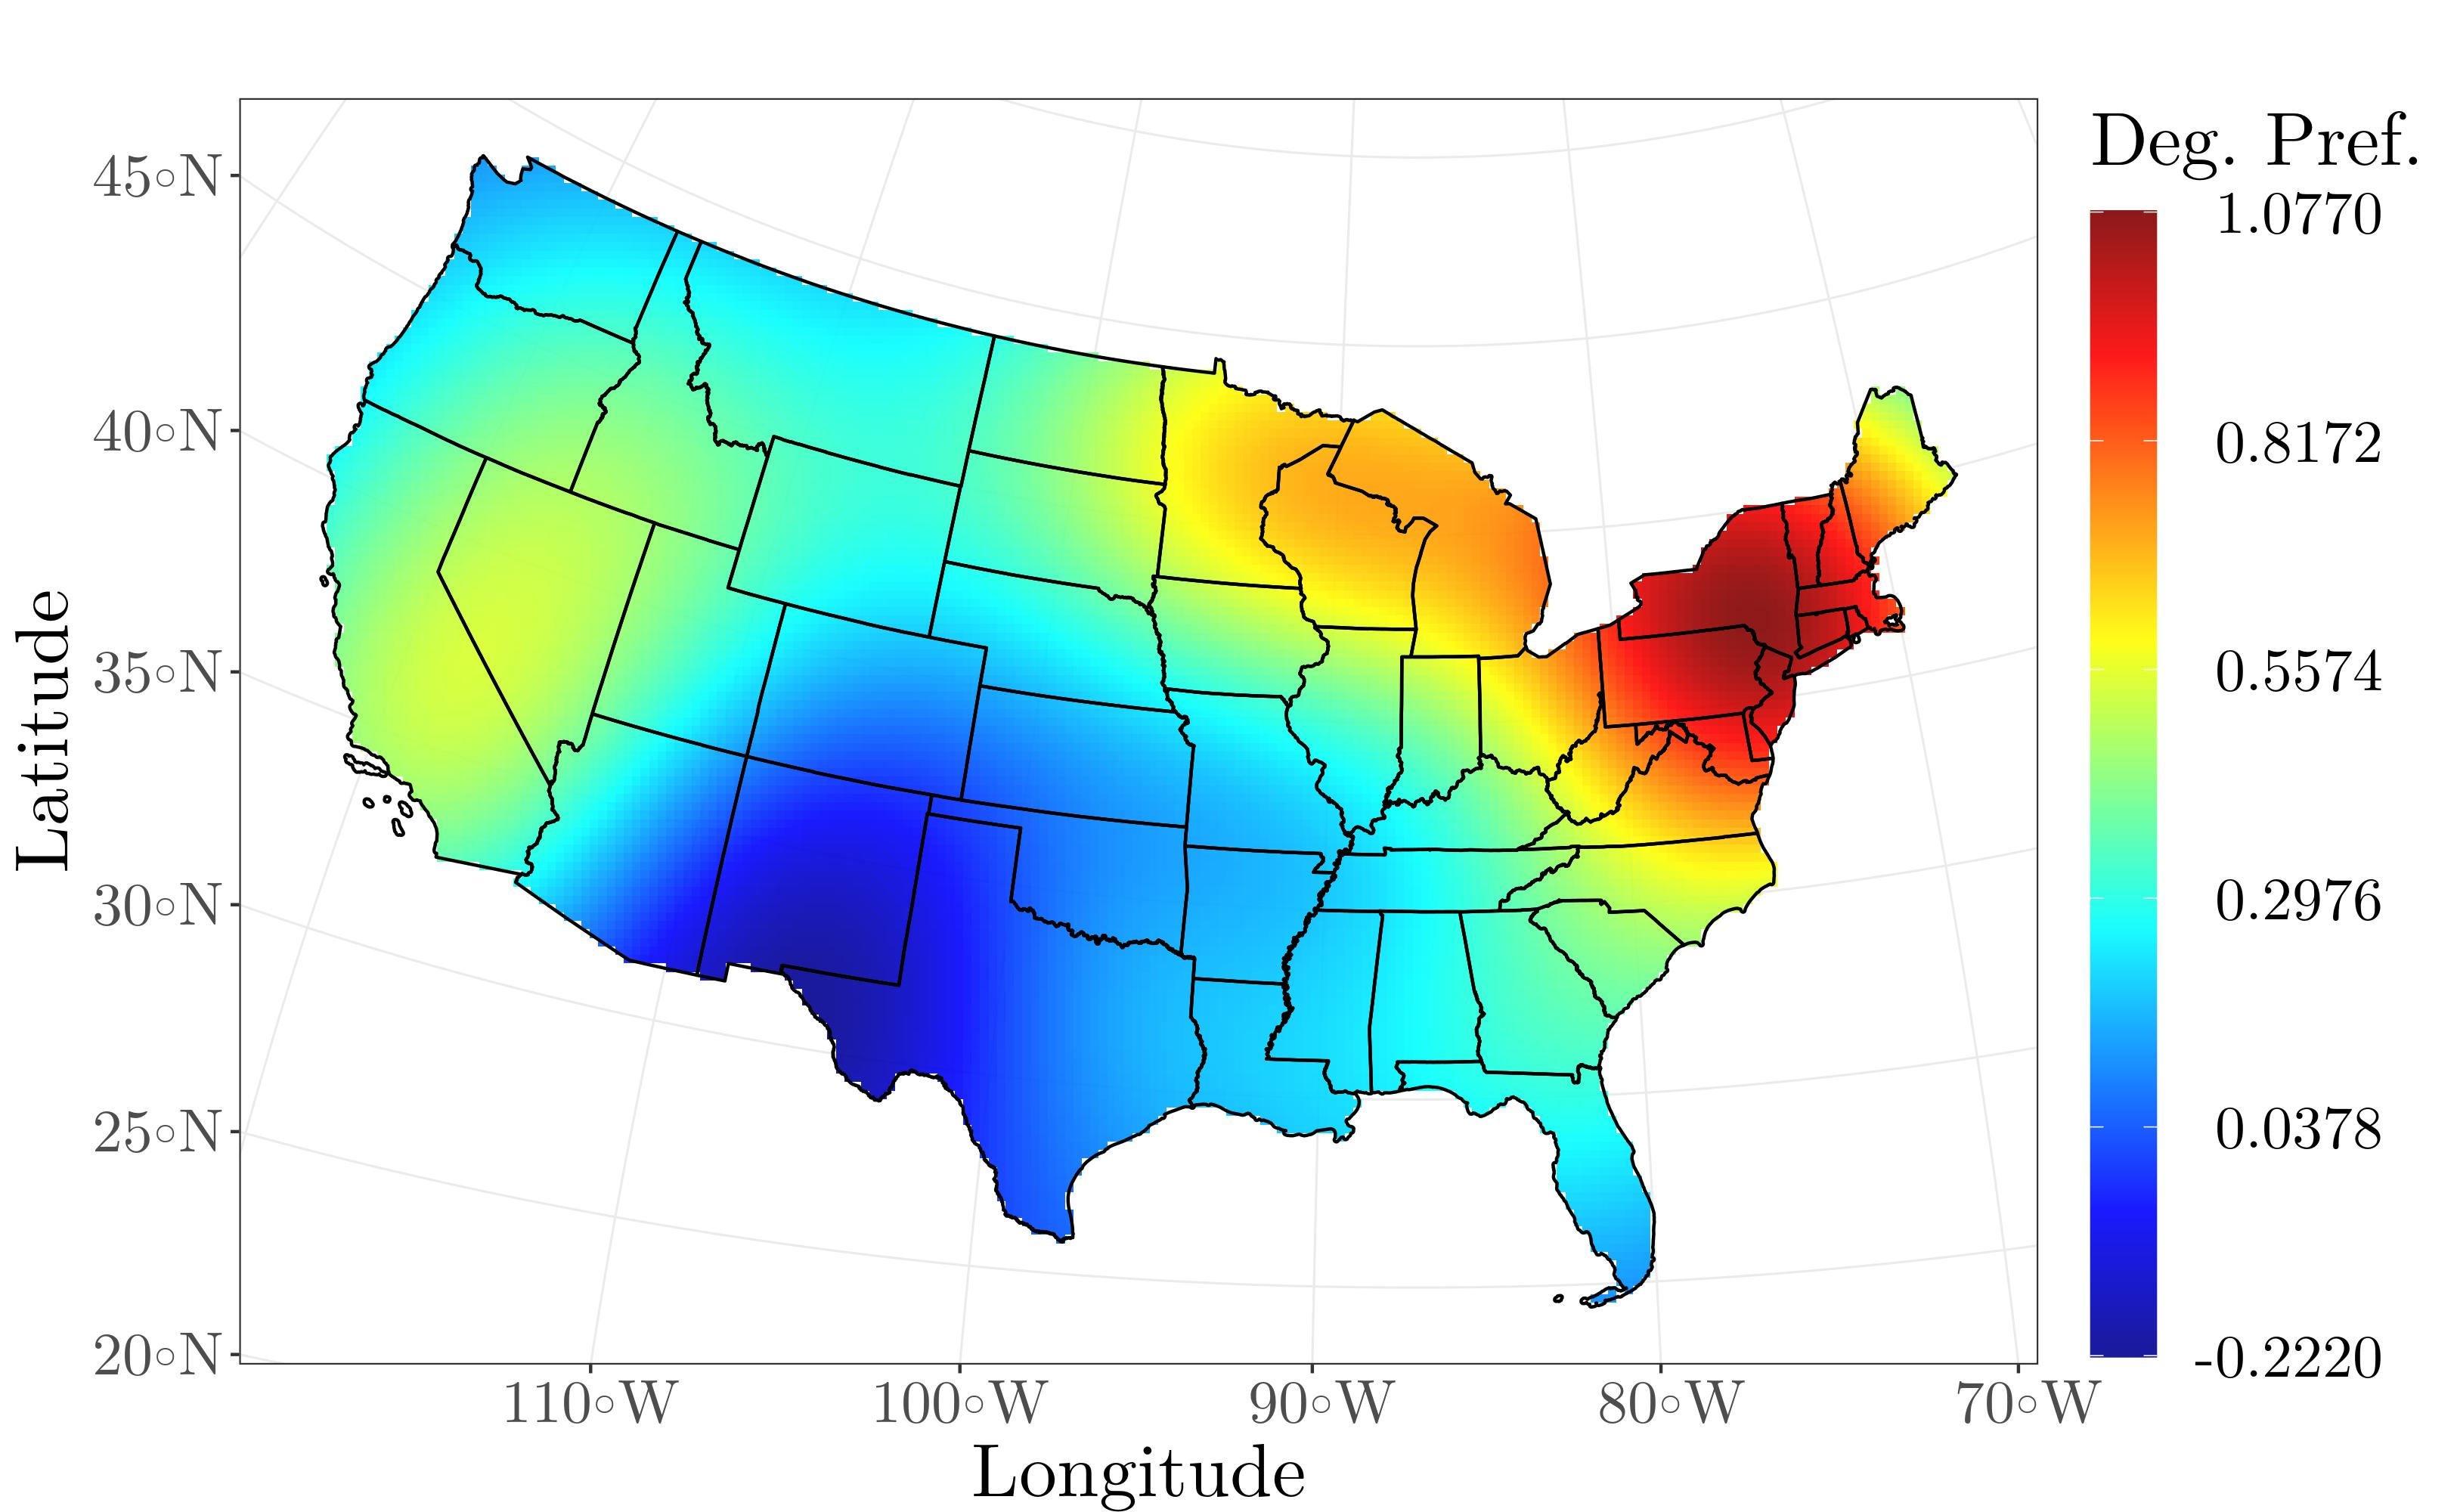
\includegraphics[width = 0.625\textwidth]{Images/preferentiality.jpeg} \vspace{-6pt}
            \caption{\justifying Estimated degree of preferentiality $\hat{\gamma}(x)$, $\forall x \in \mathscrsfs{D} = \text{USA}$, based on $\text{PM}_{2.5}$ data.}
        	\label{fig:preferentiality_usa}
        \end{figure}
    
	\end{frame}

    \begin{frame}[t]
        \frametitle{Application}
		\justifying

        As a remark, we can also investigate the estimated (based on the posterior mean) the estimated \textbf{intensity process} $\lambda(x)$.
        
        \vspace{-6pt}

        \begin{figure}[!ht]
        	\centering
        	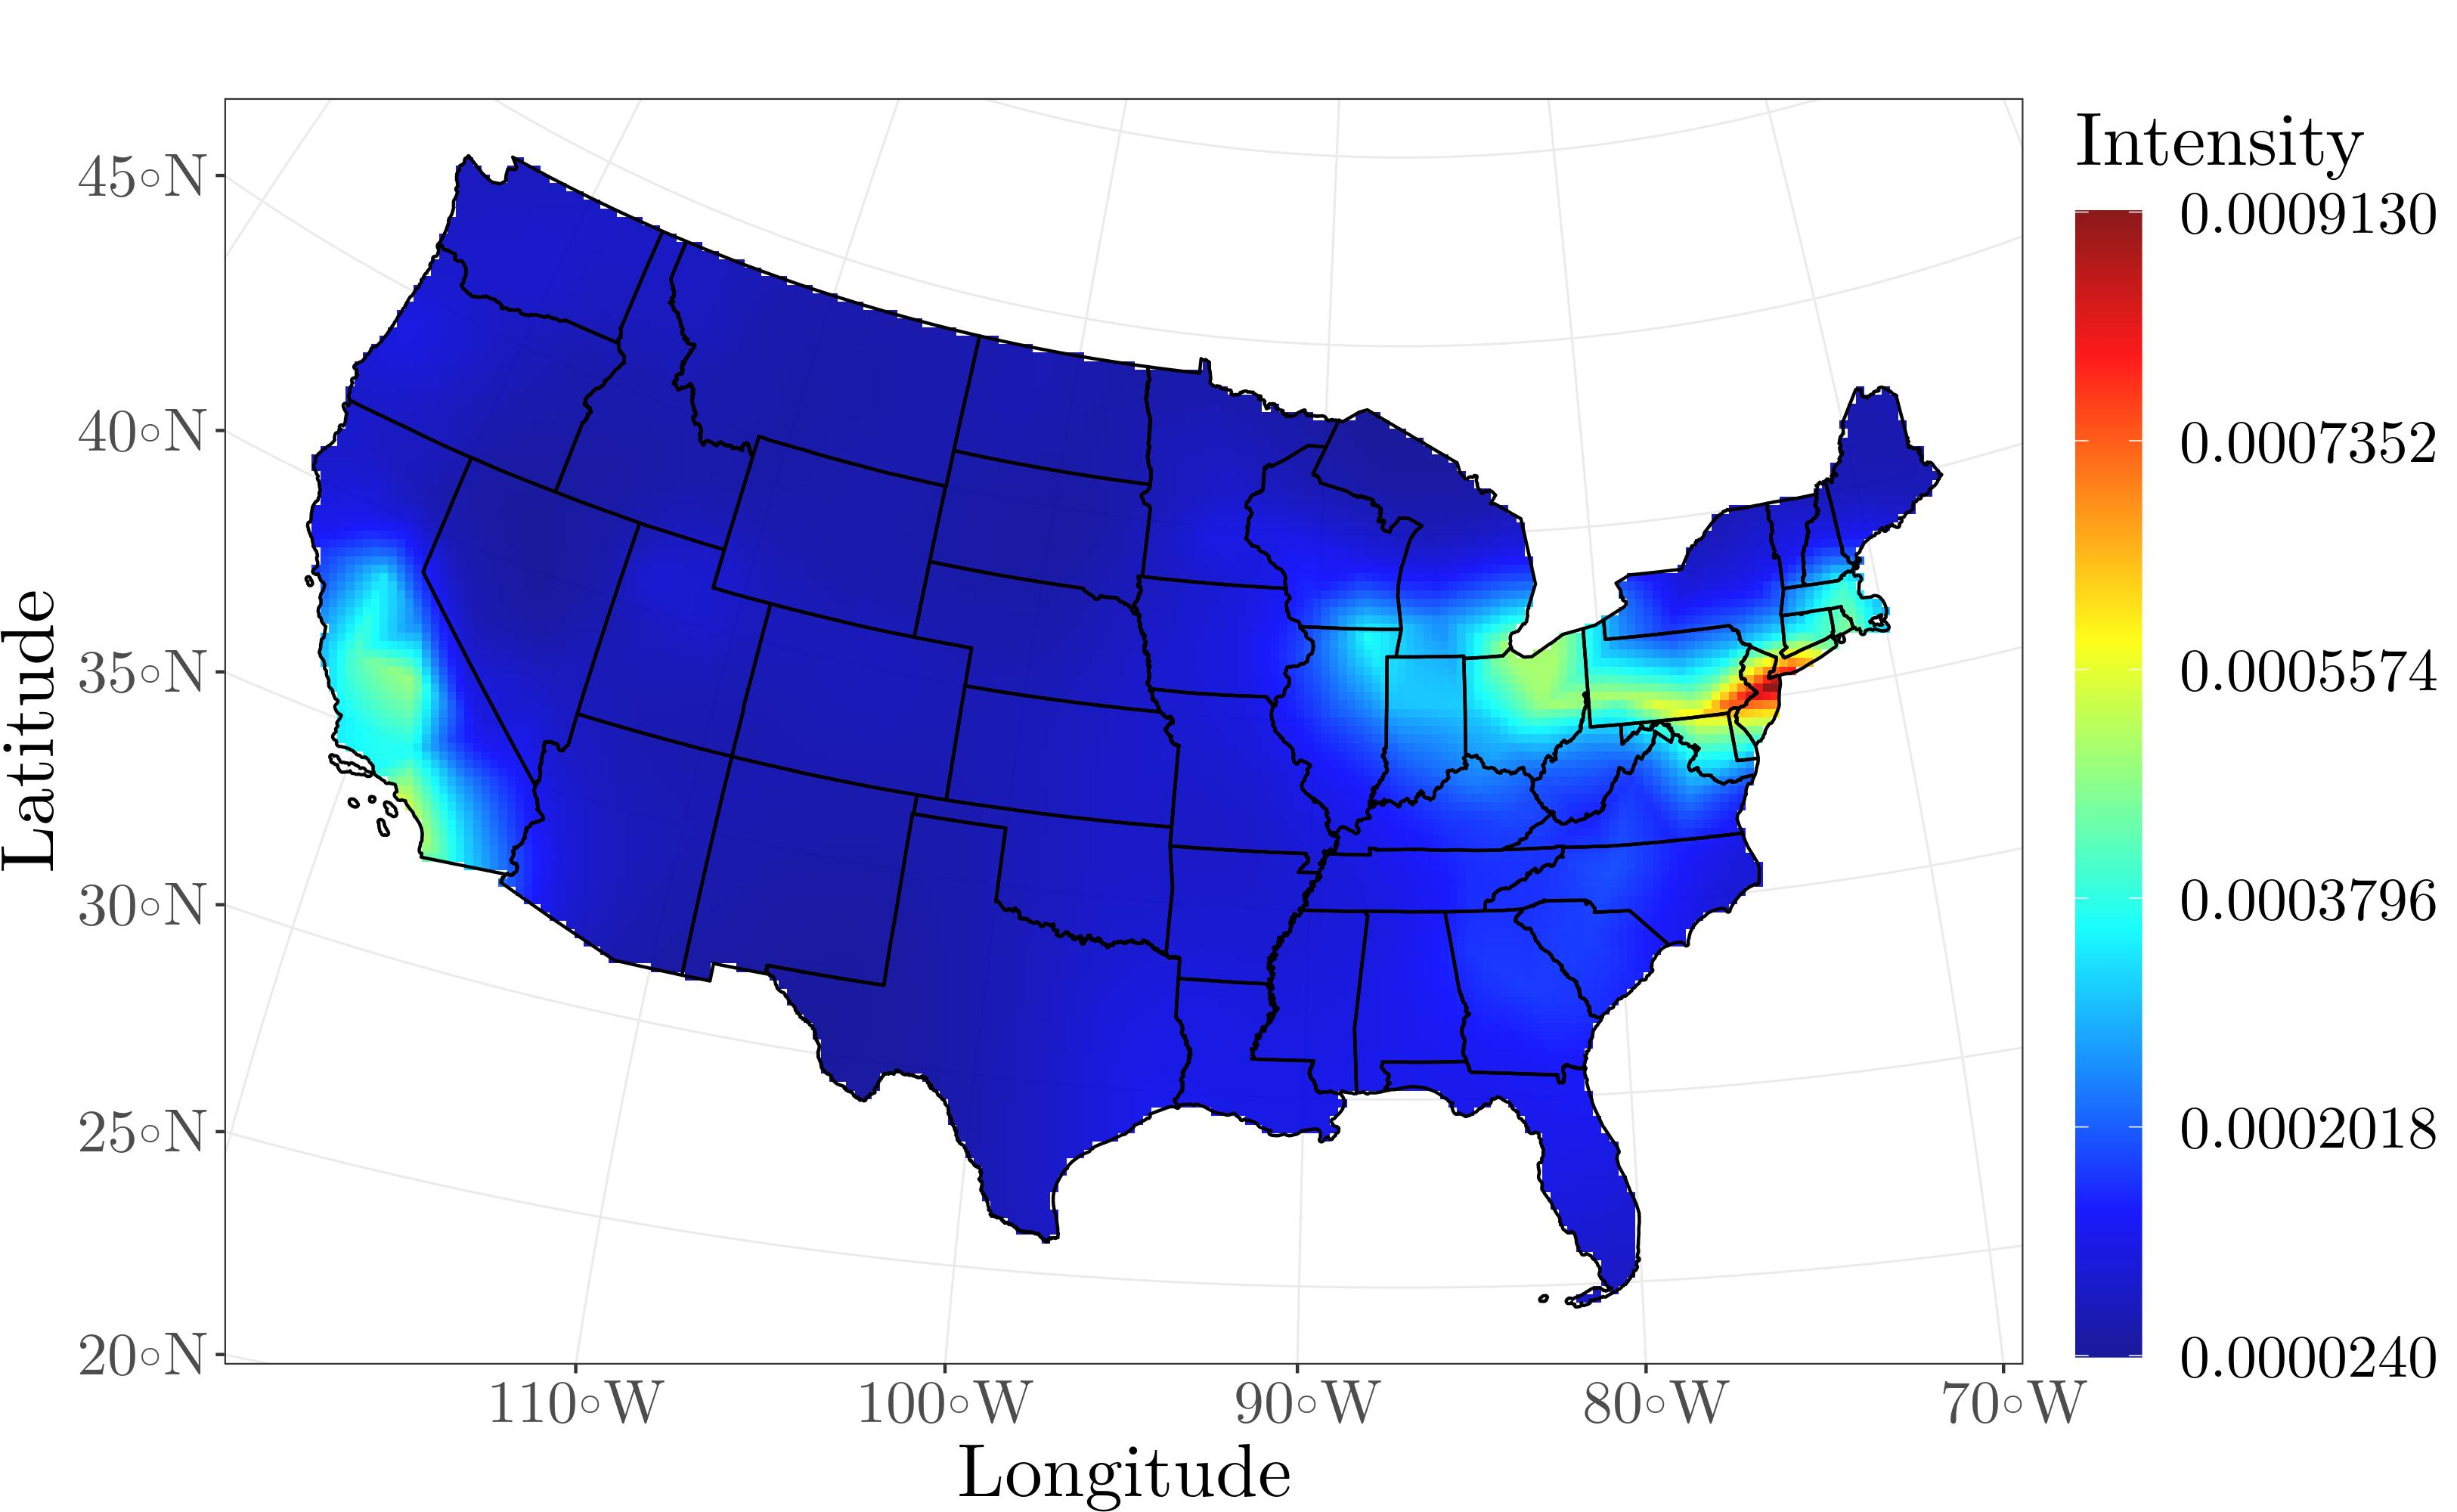
\includegraphics[width = 0.625\textwidth]{Images/intensity.jpeg} \vspace{-6pt}
            \caption{Estimated intensity process $\hat{\lambda}(x)$, $\forall x \in \mathscrsfs{D} = \text{USA}$, based on $\text{PM}_{2.5}$ data.}
        	\label{fig:S-intensity_usa}
        \end{figure}
        
	\end{frame}

     \begin{frame}[t]
        \frametitle{Discussion}
		\justifying

        We proposed a geostatistical model that accounts for spatially varying \textbf{preferential sampling} by allowing the \textbf{degree of preferentiality $\gamma(x)$ to vary over space}.

        \vspace{4pt} \pause
        
        To do so, we approximated $\gamma(x)$ by a set of \textbf{basis functions} and \hspace{2pt}\textbf{unknown coefficients}.

        \vspace{4pt} \pause

        Although I skipped the details, we implemented the model-fitting routines with the \textbf{INLA} and \textbf{SPDE} approaches which \textbf{reduces the computational burden} for parameter estimation and allows fast inference.

        \vspace{4pt} \pause

        We \textbf{concluded} that, given enough events, \textbf{our model}, along with the implemented inference routine, might \textbf{retrieve well} the latent field itself and the spatially varying preferentiality surface, (sometimes) \textbf{even under misspecified scenarios}. 

        \vspace{4pt} \pause

        As a \textit{final remark}, in the corresponding paper, we offer \textbf{guidelines} for the \textbf{specification} and \textbf{size} of the set of basis functions.
        
	\end{frame}

\end{document}